\documentclass[a4paper]{report}

\usepackage{natbib}
\bibpunct{[}{]}{,}{a}{}{;}
\usepackage{fancyheadings}
\usepackage{iamdip}

% Math packages
\usepackage{amsthm}
\usepackage{amssymb}
\usepackage{mathtools}
\usepackage{amsfonts}
\usepackage{amsmath}

% Display urls and clickable hyperlinks
\usepackage{url}
\usepackage{hyperref}

% Packages for graphics and plots
\usepackage[pdftex]{graphicx}
\usepackage{subfigure}
\usepackage{listings}
\usepackage{pdfpages}
\usepackage{asymptote}
\usepackage{tikz}
\usepackage{tikz-3dplot}
\usepackage{pgfplots}
\usetikzlibrary{intersections}
\usepackage{standalone}

% Quotation
\usepackage{dirtytalk}


\headrulewidth 0.5pt \addtolength{\headheight}{5pt}

\lhead[\fancyplain{}{\rm\thepage}]{\fancyplain{}{\rightmark}}
\rhead[\fancyplain{}{\leftmark}]{\fancyplain{}{\rm\thepage}}
\cfoot{}

\graphicspath{{../Figures/}}

\begin{document}

\pagestyle{fancyplain} \thispagestyle{empty}

\title{Attenuation-based Light Field Displays}
\author{Adrian W\"alchli}
\betreuer{Prof. Dr. Matthias Zwicker}
\ort{Bern}
\datum{2015}

\pagenumbering{roman} \setcounter{page}{1}
\maketitle

\newpage
\thispagestyle{empty}
\vspace{8cm}
\noindent
{\centerline {\bf \large Abstract}}
\vspace{1cm}
\noindent

Abstract goes here



\pagenumbering{roman} \setcounter{page}{1}
\tableofcontents

\newpage{\pagestyle{empty} \cleardoublepage}

% Hauptdokument
\pagenumbering{arabic} \setcounter{page}{1}
\pagestyle{fancy}

\chapter{Introduction}
%TODO: Figures: Lytro camera, Stanford camera array, Tensor Display etc.

\section{Related Work}

\newpage{\pagestyle{empty} \cleardoublepage}

\chapter{Capturing a Light Field}

\section{The Plenoptic Function and the Light Field}

The plenoptic function, as introduced by~\cite{AdelsonBergen}, is a 7D function that describes the intensity of light for every frequency, along every light ray in space, at any time. 
It is defined as
\begin{align*}
	P \colon \mathbb{R}^3 \times \left[0, 2 \pi \right) \times \left[ 0, \pi \right] \times \mathbb{R}^2 & \to \mathbb{R}^+ \\
	\left(x, y, z, \theta, \phi, t, \lambda \right) & \mapsto P\left(x, y, z, \theta, \phi, t, \lambda \right), 
\end{align*}
where the parameters $\left(x, y, z\right)$ are the coordinates of a point in 3D space and the angles $\left(\theta, \phi \right)$ describe the direction of an incoming light ray at time $t$. 
The light's intensity is given for every wavelength $\lambda$ and thus, the plenoptic function not only captures the visible frequency spectrum but all electromagnetic waves. 
A commonly used measure for light is the radiance, which is obtained from P by integrating over all wavelengths: 
$R\left(x, y, z, \theta, \phi, t\right) = \int_{\mathbb{R}} \! P\left(x, y, z, \theta, \phi, t, \lambda \right) \, \mathrm{d} \lambda$.

In practice, it is impossible to acquire all the data needed to model the 7D plenoptic function and hence it is reasonable to consider only a subset of the parameters. 
Dropping the time parameter $t$ in $R\left( x, y, z, \theta, \phi, t \right) $ yields a 5D function for the radiance in a static scene. 
As described by~\cite{LightFieldRendering}, this five dimensional representation can further be reduced to four dimensions in the following way. 
The radiance along a line is constant in free space and so, the 5D plenoptic function holds redundant information for the points on this line. 
Ignoring this redundancy leads to the equivalent 4D parameterization of the ray space. 
\cite{LightFieldRendering} propose a parameterization by two parallel planes, as seen in figure~\ref{fig:LightFieldParametrization}, where the coordinates of the lines (rays) are given by the intersections with the two planes.
The \textbf{4D light field} $L(u, v, s, t)$ is therefore defined as the radiance along the line intersecting the two planes at coordinates $(u, v)$ and $(s, t)$.
This two plane parameterization of the light field is the most common one seen in literature, but there are many ways to choose a parameterization.
For instance, one can use a plane and two angles to define each ray passing this plane, which would result in a light field $L(u, v, \theta, \phi)$ where $\theta, \phi \in (0, \pi)$.

\section{Light Field Acquisition}
% Figure epipolar image
% Explain epipolar images: line slope <-> depth

For practical applications, the light field must be discretized and so an appropriate sampling method needs to be chosen.
One way is to capture the light field with a grid of optical systems, e.g. cameras.
Typically, the $(u, v)$-plane is uniformly sampled on a grid $G_{uv} = \left \{ \left( u_i, v_j \right) \mid i = 1,\dots, n, j = 1, \dots, m\right \}$ on the $(u, v)$-plane with a resolution $n \times m$.
The extent in horizontal (vertical) direction is called the horizontal (vertical) \textbf{baseline}.
This means that only a slice of the actual light field can be captured and the two planes are clipped to form a rectangle.

%There are different methods to sample a light field. In principle, every camera can be used to capture 

%The samples on the $(u, v)$-plane correspond to the virtual positions of the camera. 
%Properties of the light field do not change under re-parameterization. 

\subsection*{Oblique Projections}
% Parameterization, Advantages, Disadvantages
% Mention Tomography
% Rotation 

Oblique projection, as shown in figure~\ref{fig:ObliqueProjection}, is a special case of orthographic projection: The parallel rays do not need to be perpendicular to the image plane of the camera.
The advantage is that there is a one-to-one correspondence between camera position and ray angle, since all rays in one camera are parallel.
This means that the angular resolution is simply the number of cameras, and the spatial resolution is the number of pixels in the image plane.
Given a light field $L(u, v, s, t)$ and the distance $d$ between the two planes, a re-parameterization $L^{\prime}(\theta, \phi, s, t)$ can be obtained according to figure~\ref{fig:ObliqueProjectionReparameterization} by the transformation
\begin{align*}
		& \theta = \arctan\left(\frac{u - s}{d}\right), & \phi = \arctan\left(\frac{v - t}{d}\right).
\end{align*}
However, this type of projection is only applicable for synthetic scenes that are rendered with a computer.
% TODO: Refer to a figure with a synthetic scene.


\subsection*{Perspective Projections}
% Figure
% Parameterization, two main types: global or relative
% Reparameterization: Orthographic <-> Perspective
% 
The angles of the rays in a light field captured by perspective projections are determined by the focal length and the sensor resolution of the camera.
For a camera light field, typically it is expected that
\begin{itemize}
	\item all cameras are placed at grid positions in $G_{uv}$ on the same plane, called the $(u, v)$-plane, 
	\item the optical axes of the cameras are parallel to the $(u, v)$-plane, 
	\item all cameras have the same intrinsic parameters (e.g. focal length).
\end{itemize}}
In this case, the focal planes of all cameras are forming the same plane. 
%This means that each ray can be represented by coordinates in each of the coordinate systems of the cameras.
%The only problem is that some rays are not captured by all


\section{Light Field Tomography}
% Derivation according to Wetzstein
% Explain linearity in log domain
% Mention other tomographic projection types
% SART and ART solvers
%

\section{Spectral Analysis}
% Introduction to fourier transform
% Explain the spectral support of LF



\begin{figure}
	\centering
	\documentclass{standalone}
\usepackage{tikz}

\begin{document}
	
	\begin{tikzpicture}[scale = 0.4]
	
		\filldraw[draw = black, fill = white] (0, 0) -- (5, -2) -- (5, 5) -- (0, 7) -- cycle;
		\filldraw[draw = black, fill = white] (9, 3) -- (14, 1) -- (14, 8) -- (9, 10) -- cycle;
		
		\draw[<-] (-3, 4) -- (1, 4);
		\draw (5, 4) -- (11, 4);
		\draw (14, 4) -- (17, 4);
		
		\node [left] at (-3, 4) {$L(u, v, s, t)$};
		
		
		\draw[fill] (1, 4) circle [radius = 0.1];
		\draw[fill] (11, 4) circle [radius = 0.1];
		
		\node[below right] at (1, 4) {$(u, v)$};
		\node[below right] at (11, 4) {$(s, t)$};
	
	\end{tikzpicture}
	
\end{document}
	\caption{Parametrization of the light field with two planes.}
	\label{fig:LightFieldParametrization}
\end{figure}

\begin{figure}
	\subfigure[]{
		\centering
		\documentclass{standalone}
\usepackage{tikz}

\begin{document}

	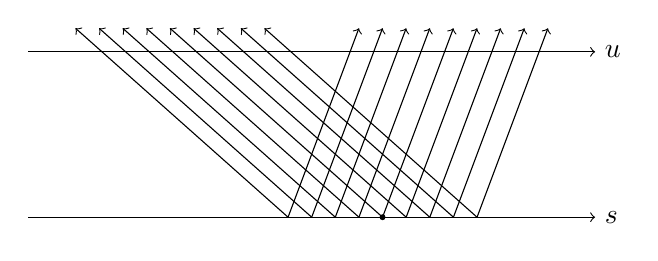
\begin{tikzpicture}[scale = 0.3, baseline]
	
		\draw[->] (-11, 0) -- (13, 0);
		\draw[->] (-11, 7) -- (13, 7);
		
		\node[right] at (13, 0) {$s$}; 
		\node[right] at (13, 7) {$u$}; 
		
		\draw[->] (0, 0) -- (-9, 8);
		\draw[->] (1, 0) -- (-8, 8);
		\draw[->] (2, 0) -- (-7, 8);
		\draw[->] (3, 0) -- (-6, 8);
		\draw[->] (4, 0) -- (-5, 8);
		\draw[->] (5, 0) -- (-4, 8);
		\draw[->] (6, 0) -- (-3, 8);
		\draw[->] (7, 0) -- (-2, 8);
		\draw[->] (8, 0) -- (-1, 8);
		
		\draw[->] (0, 0) -- (3, 8);
		\draw[->] (1, 0) -- (4, 8);
		\draw[->] (2, 0) -- (5, 8);
		\draw[->] (3, 0) -- (6, 8);
		\draw[->] (4, 0) -- (7, 8);
		\draw[->] (5, 0) -- (8, 8);
		\draw[->] (6, 0) -- (9, 8);
		\draw[->] (7, 0) -- (10, 8);
		\draw[->] (8, 0) -- (11, 8);
		
		\draw[fill] (4, 0) circle [radius = 0.1];
		
		%		\draw (0, 0) -- (0, {-sqrt(81/49 + 1)});
		%		\draw (0, 0) -- (9/7, -1);
		%		\draw (0, -1) arc (-90 : -90 + atan(9/7) : 1);
		%		
		%		\node[below right] at (0, 0) {$\theta$};
	\end{tikzpicture}

\end{document}
		\label{fig:ObliqueProjection}
	}
	\hfill
	\subfigure[]{
		\centering
		\documentclass{standalone}
\usepackage{tikz}

\usetikzlibrary{intersections}

\begin{document}
	
	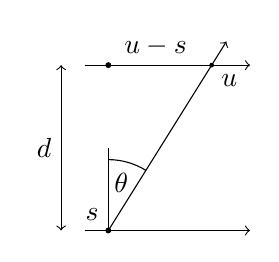
\begin{tikzpicture}[scale = 0.3, baseline]
	
		\draw[->] (-1, 0) -- (6, 0);
		\draw[name path=uAxis, ->] (-1, 7) -- (6, 7);
		
		\draw[name path=ray, ->] (0, 0) -- (5, 8);
		\node[above left] {$s$};
		
		\draw[fill] (0, 0) circle [radius = 0.1];
		\draw[fill] (0, 7) circle [radius = 0.1];
		
		\fill[name intersections={of=uAxis and ray, total=\t}]
		\foreach \s in {1,...,\t}{(intersection-\s) circle[radius = 0.1] node[below right] {$u$}};
		
		\draw (0, 0) -- (0, 3.5);
		\draw (0, 3) arc (90 : 90 - atan(5/8) : 3);
		\node at (0.55, 2) {$\theta$};
		
		\node[above] at (2, 7) {$u - s$};
		
		\draw[<->] (-2, 0) -- (-2, 7);
		\node[left] at (-2, 3.5) {$d$};
	
	\end{tikzpicture}
	
\end{document}
		\label{fig:ObliqueProjectionReparameterization}
	}
	\caption{(a) Light field aquisition using oblique projection. (b) Re-parameterization of the two-plane representation to angular coordinates.}
\end{figure}

\begin{figure}
	\subfigure[]{
		\centering
		\documentclass{standalone}
\usepackage{tikz}

\begin{document}
	
	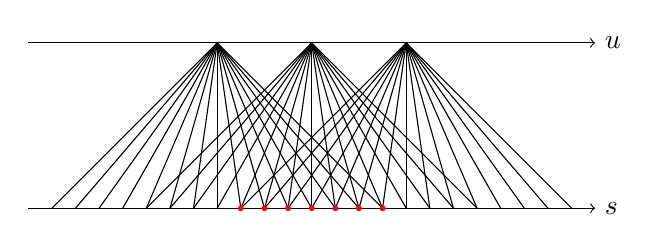
\begin{tikzpicture}[scale = 0.3]
		
		\draw[->] (-9, 0) -- (15, 0);
		\draw[->] (-9, 7) -- (15, 7);
		
		\node[right] at (15, 0) {$s$};
		\node[right] at (15, 7) {$u$};
		
		\draw (-1, 7) -- (-8, 0);
		\draw (-1, 7) -- (-7, 0);
		\draw (-1, 7) -- (-6, 0);
		\draw (-1, 7) -- (-5, 0);
		\draw (-1, 7) -- (-4, 0);
		\draw (-1, 7) -- (-3, 0);
		\draw (-1, 7) -- (-2, 0);
		\draw (-1, 7) -- (-1, 0);
		\draw (-1, 7) -- (0, 0);
		\draw (-1, 7) -- (1, 0);
		\draw (-1, 7) -- (2, 0);
		\draw (-1, 7) -- (3, 0);
		\draw (-1, 7) -- (4, 0);
		\draw (-1, 7) -- (5, 0);
		\draw (-1, 7) -- (6, 0);
		
		\draw (3, 7) -- (-4, 0);
		\draw (3, 7) -- (-3, 0);
		\draw (3, 7) -- (-2, 0);
		\draw (3, 7) -- (-1, 0);
		\draw (3, 7) -- (0, 0);
		\draw (3, 7) -- (1, 0);
		\draw (3, 7) -- (2, 0);
		\draw (3, 7) -- (3, 0);
		\draw (3, 7) -- (4, 0);
		\draw (3, 7) -- (5, 0);
		\draw (3, 7) -- (6, 0);
		\draw (3, 7) -- (7, 0);
		\draw (3, 7) -- (8, 0);
		\draw (3, 7) -- (9, 0);
		\draw (3, 7) -- (10, 0);
		
		\draw (7, 7) -- (0, 0);
		\draw (7, 7) -- (1, 0);
		\draw (7, 7) -- (2, 0);
		\draw (7, 7) -- (3, 0);
		\draw (7, 7) -- (4, 0);
		\draw (7, 7) -- (5, 0);
		\draw (7, 7) -- (6, 0);
		\draw (7, 7) -- (7, 0);
		\draw (7, 7) -- (8, 0);
		\draw (7, 7) -- (9, 0);
		\draw (7, 7) -- (10, 0);
		\draw (7, 7) -- (11, 0);
		\draw (7, 7) -- (12, 0);
		\draw (7, 7) -- (13, 0);
		\draw (7, 7) -- (14, 0);
		
		\draw[fill, red] (0, 0) circle [radius = 0.1];
		\draw[fill, red] (1, 0) circle [radius = 0.1];
		\draw[fill, red] (2, 0) circle [radius = 0.1];
		\draw[fill, red] (3, 0) circle [radius = 0.1];
		\draw[fill, red] (4, 0) circle [radius = 0.1];
		\draw[fill, red] (5, 0) circle [radius = 0.1];
		\draw[fill, red] (6, 0) circle [radius = 0.1];
	\end{tikzpicture}
	
\end{document}
		\label{fig:ShiftedPerspectiveProjection}
	}
	\hfill
	\subfigure[]{
		\centering
		\documentclass{standalone}
\usepackage{tikz}

\begin{document}
	
	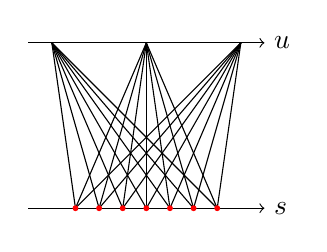
\begin{tikzpicture}[scale = 0.3]
		
		\draw[->] (-2, 0) -- (8, 0);
		\draw[->] (-2, 7) -- (8, 7);
		
		\node[right] at (8, 0) {$s$};
		\node[right] at (8, 7) {$u$};
		
		\draw (-1, 7) -- (0, 0);
		\draw (-1, 7) -- (1, 0);
		\draw (-1, 7) -- (2, 0);
		\draw (-1, 7) -- (3, 0);
		\draw (-1, 7) -- (4, 0);
		\draw (-1, 7) -- (5, 0);
		\draw (-1, 7) -- (6, 0);
		
		\draw (3, 7) -- (0, 0);
		\draw (3, 7) -- (1, 0);
		\draw (3, 7) -- (2, 0);
		\draw (3, 7) -- (3, 0);
		\draw (3, 7) -- (4, 0);
		\draw (3, 7) -- (5, 0);
		\draw (3, 7) -- (6, 0);
		
		\draw (7, 7) -- (0, 0);
		\draw (7, 7) -- (1, 0);
		\draw (7, 7) -- (2, 0);
		\draw (7, 7) -- (3, 0);
		\draw (7, 7) -- (4, 0);
		\draw (7, 7) -- (5, 0);
		\draw (7, 7) -- (6, 0);
		
		\draw[fill, red] (0, 0) circle [radius = 0.1];
		\draw[fill, red] (1, 0) circle [radius = 0.1];
		\draw[fill, red] (2, 0) circle [radius = 0.1];
		\draw[fill, red] (3, 0) circle [radius = 0.1];
		\draw[fill, red] (4, 0) circle [radius = 0.1];
		\draw[fill, red] (5, 0) circle [radius = 0.1];
		\draw[fill, red] (6, 0) circle [radius = 0.1];
		
	\end{tikzpicture}
	
\end{document}
		\label{fig:ShearedPerspectiveProjection}
	}
	\caption{Perspective projections of a scene. (a) Shifted Projection (b) Sheared projection.}
\end{figure}



\newpage{\pagestyle{empty} \cleardoublepage}


\begin{appendix}
\chapter{ap1}
\section{apsec1}
\newpage{\pagestyle{empty} \cleardoublepage}
\end{appendix}

\addcontentsline{toc}{chapter}{\numberline{}List of Tables}
\listoftables

\addcontentsline{toc}{chapter}{\numberline{}List of Figures}
\listoffigures

\addcontentsline{toc}{chapter}{\numberline{}Bibliography}
\bibliographystyle{alphadin}
\nocite{*}
\bibliography{thesis}

% This is required since 2012!!
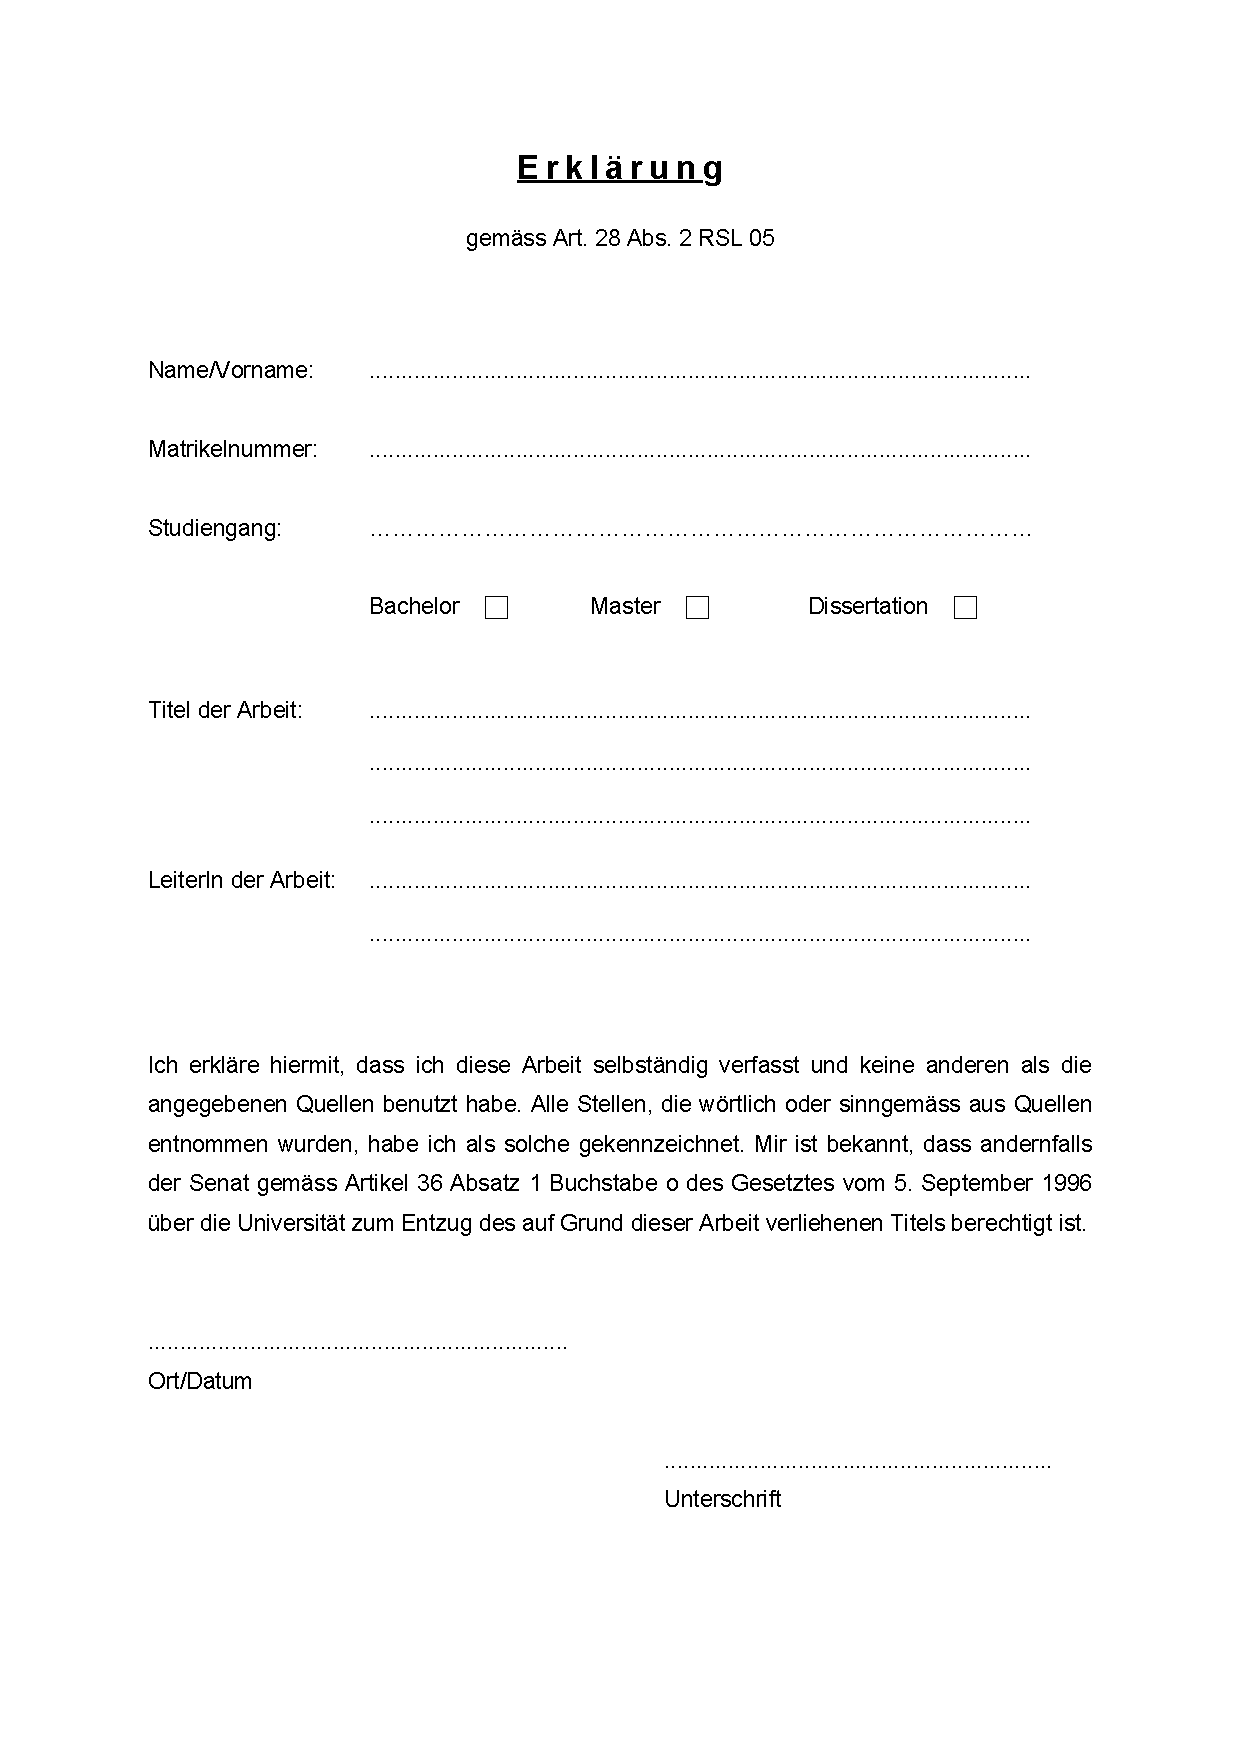
\includepdf{Erklaerung.pdf}

\end{document}
